%==============================================================================
% Chapitre 60 - Les chargements de grenaille
%==============================================================================

\section{Introduction}

La grenaille constitue la charge la plus couramment utilisée dans les cartouches
destinées au petit gibier.

Elle est composée d'un grand nombre de projectiles sphériques dont les
caractéristiques peuvent varier selon l'usage recherché.

\begin{aretenir}

Le choix de la grenaille influence directement la densité de la gerbe,
la portée utile et l'énergie des projectiles.

\end{aretenir}

\section{Principe général}

Une cartouche à grenaille contient généralement plusieurs dizaines, voire
plusieurs centaines de projectiles.

Tous ces projectiles sont propulsés simultanément lors du tir.

\section{Pourquoi utiliser de nombreux projectiles ?}

La multiplication des projectiles permet d'augmenter les probabilités
d'atteindre une cible de petite taille ou en mouvement.

Cette approche diffère fondamentalement des munitions à projectile unique.

\section{Numérotation de la grenaille}

La grenaille est généralement classée selon un système de numérotation.

Cette numérotation permet d'identifier la taille approximative des projectiles.

\section{Relation entre numéro et diamètre}

Selon la convention habituellement utilisée :

\begin{itemize}
    \item les petits numéros correspondent à de gros projectiles ;
    \item les grands numéros correspondent à de petits projectiles.
\end{itemize}

Cette logique rappelle celle des calibres de chasse.

\section{Influence du diamètre}

Le diamètre des projectiles influence notamment :

\begin{itemize}
    \item leur masse ;
    \item leur énergie ;
    \item leur vitesse résiduelle ;
    \item leur portée utile.
\end{itemize}

\section{Petite grenaille}

La petite grenaille permet de charger un grand nombre de projectiles dans une
cartouche.

Elle produit généralement des gerbes plus denses.

\section{Grande grenaille}

La grande grenaille contient moins de projectiles pour une masse totale donnée.

Chaque projectile possède toutefois davantage d'énergie.

\begin{figure}[htbp]
\centering

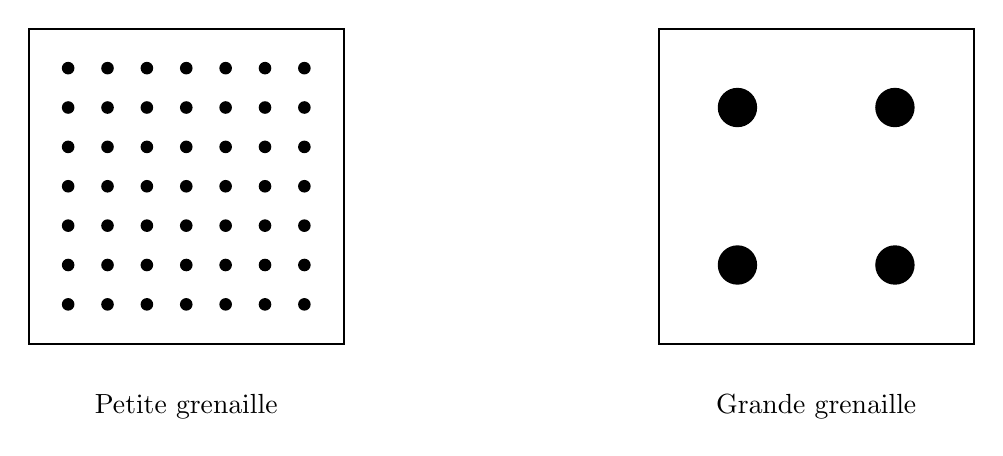
\begin{tikzpicture}

% Petite grenaille
\draw[thick] (0,0) rectangle (4,4);

\foreach \x in {0.5,1.0,1.5,2.0,2.5,3.0,3.5}
{
    \foreach \y in {0.5,1.0,1.5,2.0,2.5,3.0,3.5}
    {
        \fill (\x,\y) circle (0.08);
    }
}

\node at (2,-0.8)
{Petite grenaille};

% Grande grenaille
\begin{scope}[xshift=8cm]

\draw[thick] (0,0) rectangle (4,4);

\foreach \x/\y in {
1/1,3/1,
1/3,3/3
}
{
    \fill (\x,\y) circle (0.25);
}

\node at (2,-0.8)
{Grande grenaille};

\end{scope}

\end{tikzpicture}

\caption{À masse comparable, une petite grenaille permet d'utiliser davantage de projectiles.}
\label{fig:petite_grande_grenaille}

\end{figure}

\section{Compromis fondamental}

Le choix de la grenaille constitue un compromis entre :

\begin{itemize}
    \item nombre de projectiles ;
    \item énergie individuelle ;
    \item portée utile ;
    \item densité de gerbe.
\end{itemize}

\begin{figure}[htbp]
\centering

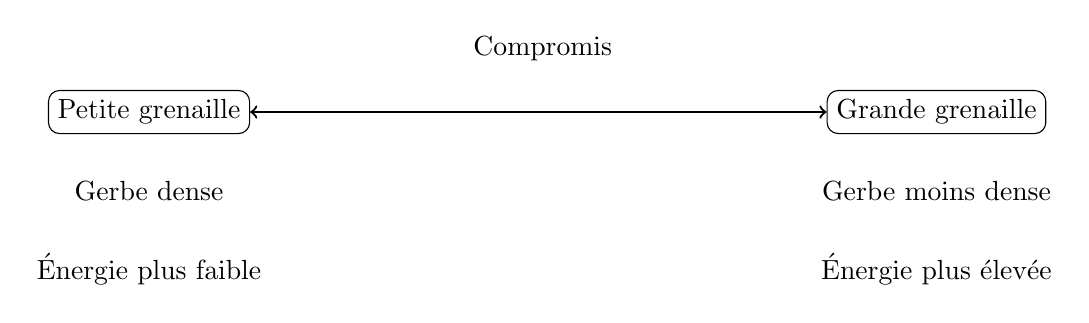
\begin{tikzpicture}

\node[draw,rounded corners]
(P)
at (-5,0)
{Petite grenaille};

\node[draw,rounded corners]
(G)
at (5,0)
{Grande grenaille};

\node
at (-5,-1)
{Gerbe dense};

\node
at (-5,-2)
{Énergie plus faible};

\node
at (5,-1)
{Gerbe moins dense};

\node
at (5,-2)
{Énergie plus élevée};

\draw[<->,thick]
(P)
--
(G);

\node at (0,0.8)
{Compromis};

\end{tikzpicture}

\caption{Compromis entre densité de gerbe et énergie individuelle des projectiles.}
\label{fig:compromis_grenaille}

\end{figure}

\section{Masse de charge}

Les cartouches de chasse sont proposées avec différentes masses de charge.

Cette masse est généralement exprimée en grammes.

\section{Influence de la masse de charge}

Lorsque la masse de charge augmente :

\begin{itemize}
    \item le nombre de projectiles augmente généralement ;
    \item le recul peut augmenter ;
    \item la densité de la gerbe peut être améliorée.
\end{itemize}

\section{Exemple de désignation}

Une cartouche peut comporter des indications telles que :

\begin{quote}
12/70 - 32 g - N°6
\end{quote}

Ces informations décrivent plusieurs caractéristiques importantes du
chargement.

\begin{figure}[htbp]
\centering

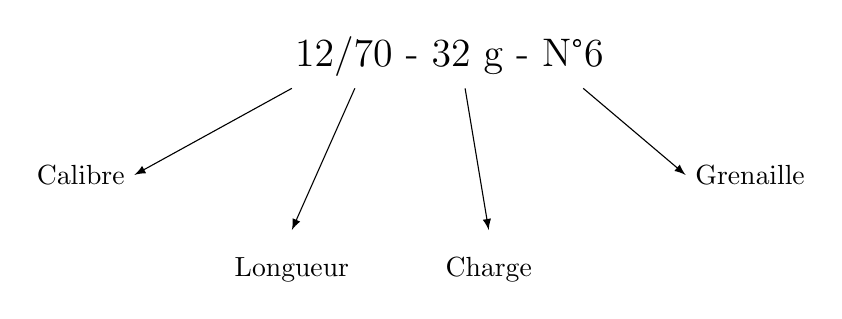
\begin{tikzpicture}

\node[font=\Large]
(T)
at (0,0)
{12/70 - 32 g - N°6};

\draw[-latex]
(-2,-0.4)
--
(-4,-1.5);

\node[left]
at (-4,-1.5)
{Calibre};

\draw[-latex]
(-1.2,-0.4)
--
(-2,-2.2);

\node
at (-2,-2.7)
{Longueur};

\draw[-latex]
(0.2,-0.4)
--
(0.5,-2.2);

\node
at (0.5,-2.7)
{Charge};

\draw[-latex]
(1.7,-0.4)
--
(3,-1.5);

\node[right]
at (3,-1.5)
{Grenaille};

\end{tikzpicture}

\caption{Exemple de lecture d'une désignation de cartouche de chasse.}
\label{fig:designation_cartouche_chasse}

\end{figure}

\section{Adaptation au gibier}

Le choix de la grenaille dépend notamment :

\begin{itemize}
    \item de la taille du gibier ;
    \item de la distance de tir ;
    \item des conditions de chasse.
\end{itemize}

\section{Influence de la distance}

À mesure que la distance augmente, les projectiles perdent progressivement
de leur énergie.

Le choix de la taille de la grenaille doit tenir compte de ce phénomène.

\begin{figure}[htbp]
\centering

\begin{tikzpicture}[scale=1]

% Axes
\draw[-latex] (0,0) -- (8,0)
node[right]
{Distance};

\draw[-latex] (0,0) -- (0,5)
node[above]
{Énergie};

% Petite grenaille
\draw[thick]
(0,4)
.. controls (2,2.5) and (4,1.2) ..
(7,0.2);

\node at (6,1)
{Petite};

% Grande grenaille
\draw[thick]
(0,4.5)
.. controls (2,3.8) and (5,2.5) ..
(7,1.5);

\node at (6,2.5)
{Grande};

\end{tikzpicture}

\caption{Illustration qualitative de l'évolution de l'énergie avec la distance.}
\label{fig:energie_grenaille_distance}

\end{figure}

\section{Matériaux utilisés}

La grenaille peut être réalisée dans différents matériaux :

\begin{itemize}
    \item plomb ;
    \item acier ;
    \item bismuth ;
    \item tungstène.
\end{itemize}

\section{Limites des généralisations}

Les performances observées dépendent de nombreux paramètres.

Les recommandations générales doivent toujours être confrontées aux essais
pratiques.

\section{Vers les chevrotines}

Toutes les charges multiples ne sont pas constituées de petite grenaille.

Le chapitre suivant examinera les chevrotines et leurs caractéristiques
particulières.

\begin{figure}[htbp]
\centering

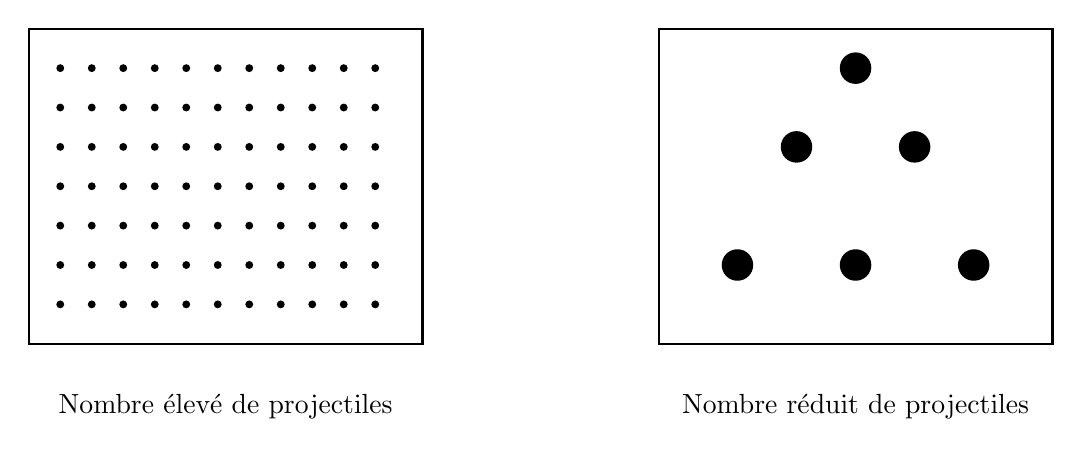
\begin{tikzpicture}

% Petite grenaille
\draw[thick] (0,0) rectangle (5,4);

\foreach \x in {0.4,0.8,1.2,1.6,2.0,2.4,2.8,3.2,3.6,4.0,4.4}
{
    \foreach \y in {0.5,1.0,1.5,2.0,2.5,3.0,3.5}
    {
        \fill (\x,\y) circle (0.05);
    }
}

\node at (2.5,-0.8)
{Nombre élevé de projectiles};

% Grande grenaille
\begin{scope}[xshift=8cm]

\draw[thick] (0,0) rectangle (5,4);

\foreach \x/\y in {
1/1,2.5/1,4/1,
1.75/2.5,3.25/2.5,
2.5/3.5
}
{
    \fill (\x,\y) circle (0.20);
}

\node at (2.5,-0.8)
{Nombre réduit de projectiles};

\end{scope}

\end{tikzpicture}

\caption{Pour une masse totale comparable, la taille des projectiles influence directement leur nombre.}
\label{fig:nombre_projectiles}

\end{figure}

\section{À retenir}

\begin{aretenir}

\begin{itemize}
    \item La grenaille est constituée d'un grand nombre de projectiles sphériques.
    \item Le diamètre influence directement les performances.
    \item Il existe un compromis entre densité de gerbe et énergie individuelle.
    \item La masse de charge constitue un paramètre important.
    \item Le choix dépend toujours de l'usage recherché.
\end{itemize}

\end{aretenir}
